% This file was converted to LaTeX by Writer2LaTeX ver. 1.6.1
% see http://writer2latex.sourceforge.net for more info
\documentclass[a4paper]{article}
\usepackage[utf8]{inputenc}
\usepackage{wrapfig}
\usepackage{amsmath}
\usepackage{amssymb,amsfonts,textcomp}
\usepackage[T1]{fontenc}
\usepackage[english,spanish]{babel}
\usepackage{color}
\usepackage{array}
\usepackage{hhline}
% Outline numbering
\setcounter{secnumdepth}{0}
% Page layout (geometry)
\setlength\voffset{-1in}
\setlength\hoffset{-1in}
\setlength\topmargin{2cm}
\setlength\oddsidemargin{2cm}
\setlength\textheight{25.7cm}
\setlength\textwidth{17.001cm}
\setlength\footskip{0.0cm}
\setlength\headheight{0cm}
\setlength\headsep{0cm}
% Footnote rule
\setlength{\skip\footins}{0.119cm}
\renewcommand\footnoterule{\vspace*{-0.018cm}\setlength\leftskip{0pt}\setlength\rightskip{0pt plus 1fil}\noindent\textcolor{black}{\rule{0.25\columnwidth}{0.018cm}}\vspace*{0.101cm}}
% Pages styles
\makeatletter
\newcommand\ps@Standard{
  \renewcommand\@oddhead{}
  \renewcommand\@evenhead{}
  \renewcommand\@oddfoot{}
  \renewcommand\@evenfoot{}
  \renewcommand\thepage{\arabic{page}}
}
\makeatother
\pagestyle{Standard}
% List styles
\newcommand\liststyleLi{%
\renewcommand\labelitemi{•}
\renewcommand\labelitemii{•}
\renewcommand\labelitemiii{•}
\renewcommand\labelitemiv{•}
}


%
\usepackage{graphicx}
\usepackage[hidelinks,breaklinks=true,backref=page]{hyperref}

\usepackage[spanish]{babel}
\usepackage[utf8]{inputenc}


\begin{document}

\title{26.El desarrollo de las redes adversariales}
\author{Luis Ernesto Ibarra Vázquez C511\and
Luis Enrique Dalmau Coopat C511}
%
%\authorrunning{F. Author et al.}
% First names are abbreviated in the running head.
% If there are more than two authors, 'et al.' is used.
%
\renewcommand{\refname}{Bibliografía} 

\maketitle

\begin{abstract}

El trabajo trata sobre los distintos tipos de redes neuronales y cómo estas fueron desarrollándose
para llegar a ser uno de los avances más importantes de Ciencias de la Computación del siglo XX y XXI.
Se prestará especial atención a las Redes Generativas Adversariales, la historia detrás de su origen y
la importancia que tiene en la actualidad, así como sus problemas y efectos curiosos que pueden ocurrir
en caso de no ser correctamente entrenadas. 

\end{abstract}

\textbf{Palabras clave}: Inteligencia Artificial(IA), Redes Neuronales, Redes Generativas Adversariales(RGA).

\textbf{Keywords}: Artifitial Inteligence(AI), Neural Networks, Generative Adversarial Networks (GAN).

\section{Introducción}

Las Redes Generativas Adversariales representan un gran paso en el desarrollo de la Inteligencia
Artificial. Estas son un caso particular de las Redes Neuronales Artificiales nacidas en el siglo XX.
Como dijo Martin Giles 
``Al enfrentar las redes neuronales entre sí, Ian Goodfellow ha creado una poderosa herramienta 
de IA. Ahora él y el resto de nosotros, debemos afrontar las consecuencias.''. Pero, para comprender 
esta frase primero debemos conocer las siguientes interrogantes. ¿Qué son y cómo surgieron las redes neuronales? 
¿Cúal es la idea detrás de las RGA (GAN por sus siglas en inglés), cómo surgieron? y por supuesto ¿Quién es Ian Goodfellow?.

\section{Antecedentes de las GAN}
Evolución de las Redes Neuronales en Ciencias de la Computación:
\begin{itemize}

    \item{1958 – Perceptrón}
    \item{1965 – Perceptrón Multicapas}
    \item{1980’s
    	\begin{itemize}
    	\item{Neuronas Sigmoidales}
        \item{Redes Feedforward}
        \item{Backpropagation}
        \end{itemize}
        }
    \item{1989 – Convolutional neural networks (CNN) / Recurent neural networks (RNN)}
    \item{1997 – Long short term memory (LSTM)}
    \item{2006 – Deep Belief Networks (DBN): Nace el deep learning}
    \begin{itemize}
    
        \item{Restricted Boltzmann Machine}
        \item{Encoder / Decoder = Auto-encoder}
        
    \end{itemize}
    \item{2014 – Generative Adversarial Networks (GAN)}

\end{itemize}

\newpage
\subsection{Perceptrón}
\begin{wrapfigure}{r}{0.15\textwidth} %this figure will be at the right
    \centering
    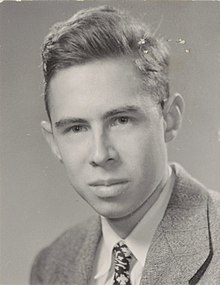
\includegraphics[width=0.15\textwidth]{./images/220px-Rosenblatt_21.jpg}
    \caption{Frank Rossenblatt}
\end{wrapfigure}

Las redes neuronales nacieron con el Perceptrón a mediados del 
siglo XX. El primer tipo de red neuronal y la menos compleja pero 
un gigantezco primer paso en la dirección correcta. Estas surgieron
entre las décadas de 1950 y 1960 cuando el científico Frank Rosenblatt, 
inspirado en el trabajo de Warren McCulloch y Walter Pitts creó el 
Perceptrón, la unidad desde donde nacerían y se potenciarían las 
redes neuronales artificiales\cite{wikipercept}.

Frank Rossenblatt (11 de julio de 1928-11 de julio de 1971) fue un
psicólogo estadounidense notable en el campo de inteligencia
artificial.En el Laboratorio Cornell Aeronáutico en Búfalo (Nueva
York), donde fue sucesivamente psicólogo investigador, psicólogo
sénior y jefe de la sección de sistemas cognitivos,
también dirigió sus primeros trabajos 
sobre perceptrones, que culminaron en el desarrollo
y construcción del hardware del 
perceptrón Mark I en 1960\cite{wikifrank}.
Este era esencialmente el primer ordenador que podría aprender 
habilidades nuevas a prueba y error, utilizando un tipo de red 
neuronal que simula el proceso de pensamiento humano. 

\begin{wrapfigure}{l}{0.2\textwidth} %this figure will be at the right
    \centering
    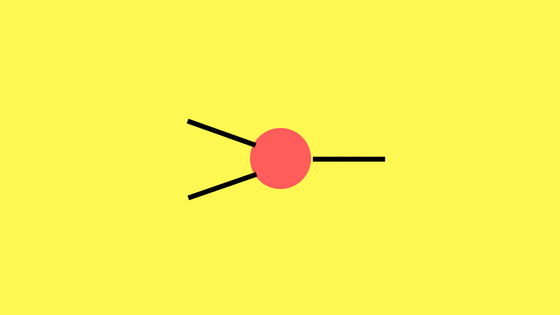
\includegraphics[width=0.2\textwidth]{./images/net_perceptron.png}
    \caption{Perceptrón}
\end{wrapfigure}

Un perceptrón toma varias entradas binarias $x_1$, $x_2$, etc y produce 
una sola salida binaria. Para calcular la salida, Rosenblatt 
introduce el concepto de ``pesos'' $w_1$, $w_2$, etc, un número real que 
expresa la importancia de la respectiva entrada con la salida. La 
salida de la neurona será 1 o 0 si la suma de la multiplicación de 
pesos por entradas es mayor o menor a un determinado umbral.
Sus principales usos son decisiones binarias sencillas, o para 
crear funciones lógicas como OR, AND. Sin embargo no podía 
resolver problemas no lineales.

\qquad

\subsection{Perceptrón Multicapas}
\begin{wrapfigure}{l}{0.25\textwidth} %this figure will be at the right
    \centering
    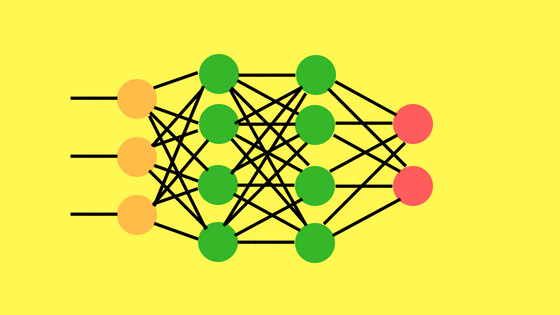
\includegraphics[width=0.25\textwidth]{./images/net_multilayer.png}
    \caption{Perceptrón Multicapas}
\end{wrapfigure}

En 1969, Minsky y Papert, demuestran que el perceptrón simple y 
ADALINE no puede resolver problemas no lineales (por ejemplo, 
XOR). La combinación de varios perceptrones simples podría 
resolver ciertos problemas no lineales pero no existía un 
mecanismo automático para adaptar los pesos de la capa oculta. 
Rumelhart y otros autores, en 1986, presentan la ``Regla Delta 
Generalizada'' para adaptar los pesos propagando los errores hacia 
atrás, es decir, propagar los errores hacia las capas ocultas 
inferiores\cite{wikimultilayer}.


De esta forma se consigue trabajar con múltiples capas y con 
funciones de activación no lineales. Se demuestra que el 
perceptrón multicapa es un aproximador universal. Un perceptrón 
multicapa puede aproximar relaciones no lineales entre los datos 
de entrada y salida. Esta red se ha convertido en una de las 
arquitecturas más utilizadas en el momento.

\subsection{Avances en los 80}

\subsubsection{Neuronas Sigmoides}
\begin{wrapfigure}{l}{0.2\textwidth} %this figure will be at the right
    \centering
    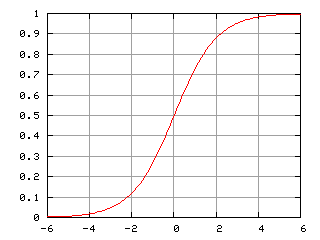
\includegraphics[width=0.2\textwidth]{./images/Logistic-curve.png}
    \caption{Función Sigmoid}
\end{wrapfigure}

Para poder lograr que las redes de neuronas aprendieran solas fue 
necesario introducir un nuevo tipo de neuronas. Las llamadas 
Neuronas Sigmoides son similares al perceptrón, pero permiten que 
las entradas, en vez de ser ceros o unos, puedan tener valores 
reales como 0,5 ó 0,377 ó lo que sea. También aparecen las 
neuronas ``bias'' que siempre suman 1 en las diversas capas para 
resolver ciertas situaciones. Ahora las salidas en vez de ser 0 ó 
1, será d(w . x + b) donde d será la función sigmoide definida 
como $d(z) = \dfrac{1}{( 1 +e^{-z})}$ . Esta sería la primera 
función de activación\cite{wikilogit}.
\\
\\
\begin{wrapfigure}{r}{0.1\textwidth} %this figure will be at the right
    \centering
    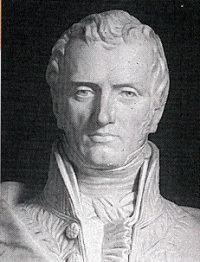
\includegraphics[width=0.1\textwidth]{./images/Pierre_Francois.jpeg}
    \caption{Pierre F.Verhulst}
\end{wrapfigure}

La función logística o sigmoidal fue desarrollada como un modelo 
de crecimiento de población y nombrada ``logística'' por Pierre 
François Verhulst en las décadas de 1830 y 1840, bajo la dirección 
de Adolphe Quetelet\cite{wikipierre}.
En su primer artículo (1838), Verhulst no especificó cómo ajustaba 
las curvas a los datos. En su artículo más detallado (1845), 
Verhulst determinó los tres parámetros del modelo haciendo que la 
curva pasara por tres puntos observados, lo que produjo una 
predicción deficiente.

Posterior a este primer descubrimiento, muchos otros autores
redescubren esta misma función en otros ámbitos, llamándolas de
diversas maneras. En química como modelo de autocatálisis (Wilhelm 
Ostwald, 1883) y redescubierto como modelo de crecimiento
demográfico en 1920 por Raymond Pearl y Lowell Reed, publicado 
como Pearl \& Reed (1920). El término ``logística'' fue revivido 
por Udny Yule en 1925 y ha sido seguido desde entonces.


Con esta nueva fórmula, se puede lograr que pequeñas alteraciones 
en valores de los pesos (deltas) produzcan pequeñas alteraciones 
en la salida. Por lo tanto, podemos ir ajustando muy de a poco los 
pesos de las conexiones e ir obteniendo las salidas deseadas.

\subsubsection{Redes Feedforward}

Se les llama así a las redes en que las salidas de una capa son 
utilizadas como entradas en la próxima capa. Esto quiere decir que 
no hay loops "hacia atrás". Siempre se "alimenta" de valores hacia 
adelante. Hay redes que veremos más adelante en las que sí que 
existen esos ciclos (Recurrent Neural Networks). Además existe el 
concepto de ``fully connected Feedforward Networks'' y se refiere 
a que todas las neuronas de entrada, están conectadas con todas las 
neuronas de la siguiente capa.

\subsubsection{Backpropagation}

Gracias al algoritmo de backpropagation se hizo posible entrenar 
redes neuronales de múltiples capas de manera supervisada. Al 
calcular el error obtenido en la salida e ir propagando hacia las 
capas anteriores se van haciendo ajustes pequeños (minimizando 
costo) en cada iteración para lograr que la red aprenda 
consiguiendo que la red pueda -por ejemplo- clasificar las 
entradas correctamente.

El termino retropropagación (backpropagation) y su uso general en 
redes neuronales se anunció en Rumelhart, Hinton \& Williams 
(1986), luego se elaboró y popularizó en Rumelhart, 
Hinton \& Williams (1986), pero la técnica se redescubrió de forma 
independiente muchas veces y tuvo muchos predecesores que datan a 
la década de 1960.

Los conceptos básicos de la retropropagación continua se derivaron 
en el contexto de la teoría del control por Henry J. Kelley en 
1960 y por Arthur E. Bryson en 1961. Utilizaron principios de 
programación dinámica. En 1962, Stuart Dreyfus publicó una 
derivación más simple basada únicamente en la regla de la cadena. 
Bryson y Ho lo describieron como un método de optimización de 
sistemas dinámicos de varias etapas en 1969. La retropropagación 
fue derivada por varios investigadores a principios de los años 60 
e implementada para ejecutarse en computadoras ya en 1970 por 
Seppo Linnainmaa. Paul Werbos fue el primero en los EE. UU. en 
proponer que podría usarse para redes neuronales después de 
analizarlo en profundidad en su disertación de 1974. Si bien no se 
aplicó a las redes neuronales, en 1970 Linnainmaa publicó el 
método general para la diferenciación automática (DA). Aunque es 
muy controvertido, algunos científicos creen que este fue en 
realidad el primer paso hacia el desarrollo de un algoritmo de 
propagación hacia atrás. En 1973, Dreyfus adapta los parámetros de 
los controladores en proporción a los gradientes de error. En 1974 
Werbos mencionó la posibilidad de aplicar este principio a redes 
neuronales artificiales, y en 1982 aplicó el método DA de 
Linnainmaa a funciones no lineales.

Posteriormente, el método Werbos fue redescubierto y descrito en 
1985 por Parker, y en 1986 por Rumelhart, Hinton y Williams. 
Rumelhart, Hinton y Williams demostraron experimentalmente que 
este método puede generar representaciones internas útiles de 
datos entrantes en capas ocultas de redes neuronales. Yann LeCun 
propuso la forma moderna del algoritmo de aprendizaje de 
retropropagación para redes neuronales en su tesis doctoral en 
1987. En 1993, Eric Wan ganó un concurso internacional de 
reconocimiento de patrones a través de retropropagación.

\subsection{Convolutional Neural Network}
\begin{wrapfigure}{l}{0.25\textwidth} %this figure will be at the right
    \centering
    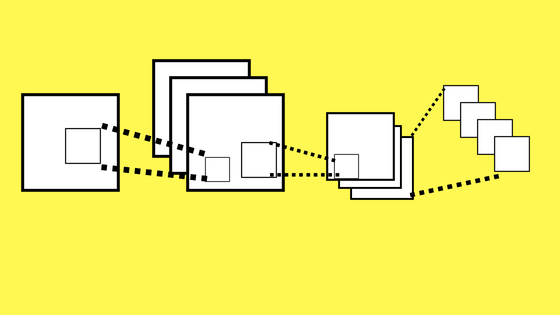
\includegraphics[width=0.25\textwidth]{./images/net_convolutional.png}
    \caption{CNN}
\end{wrapfigure}

Las Convolutional Neural Networks (CNN) o Redes Neuronales Convolucionales 
son redes multilayered que toman 
su inspiración del cortex visual de los animales. Esta 
arquitectura es útil en varias aplicaciones, principalmente 
procesamiento de imágenes. La primera CNN fue creada por Yann 
LeCun y estaba enfocada en el reconocimiento de letras 
manuscritas.

\begin{wrapfigure}{r}{0.25\textwidth} %this figure will be at the right
    \centering
    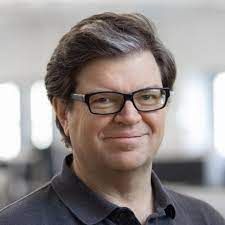
\includegraphics[width=0.25\textwidth]{./images/Yann_LeCun.jpeg}
    \caption{Yann LeCun}
\end{wrapfigure}

Yann André LeCun (nacido el 8 de julio de 1960) es un informático 
franco-estadounidense que trabaja principalmente en los campos del 
aprendizaje automático , visión por computadora, robótica móvil y 
neurociencia computacional. Es profesor de plata del Courant 
Institute of Mathematical Sciences de la Universidad de Nueva York 
y vicepresidente, científico jefe de IA en Meta ( Anteriormente 
Facebook )\cite{wikiyann}.
\newpage
Es conocido por su trabajo en reconocimiento óptico de caracteres 
y visión por computadora utilizando redes neuronales 
convolucionales, y es el padre fundador de redes 
convolucionales. También es uno de los principales creadores de la 
tecnología de compresión de imagen DjVu (junto con Léon Bottou y 
Patrick Haffner). Co-desarrolló el lenguaje de programación Lush 
con Léon Bottou. Es además co-receptor del Premio Turing en 2018 de la ACM junto con 
Geoffrey Hinton y Yoshua Bengio por su trabajo en aprendizaje 
profundo. LeCun, junto con Hinton y Bengio, son conocidos por algunos como 
los ``Padrinos de la IA'' y ``Padrinos del Aprendizaje Profundo''. 

La arquitectura de la primera CNN constaba de varias capas que 
implementaban la extracción de características y luego clasificar. 
La imagen se divide en campos receptivos que alimentan una capa 
convolutional que extrae features de la imagen de entrada (Por 
ejemplo, detectar lineas verticales, vértices, etc). El siguiente 
paso es pooling que reduce la dimensionalidad de las features 
extraídas manteniendo la información más importante. Luego se hace 
una nueva convolución y otro pooling que alimenta una red 
feedforward multicapa. La salida final de la red es un grupo de 
nodos que clasifican el resultado, por ejemplo un nodo para cada 
número del 0 al 9 (es decir, 10 nodos, se ``activan'' de a uno).

Esta arquitectura usando capas profundas y la clasificación de 
salida abrieron un mundo nuevo de posibilidades en las redes 
neuronales. Las CNN se usan también en reconocimiento de video y 
tareas de Procesamiento del Lenguaje natural. 


\subsection{Long Short Term Memory / Recurrent Neural Network}
\begin{wrapfigure}{l}{0.25\textwidth} %this figure will be at the right
    \centering
    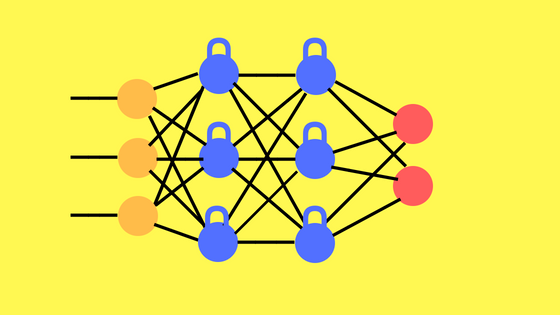
\includegraphics[width=0.25\textwidth]{./images/net_lstm.png}
    \caption{LSTM}
\end{wrapfigure}

Las Long Short Term Memory (LSTM) son un tipo de Recurrent neural 
network. Esta arquitectura permite conexiones ``hacia atrás'' entre 
las capas. Esto las hace buenas para procesar datos de tipo "time 
series" (datos históricos). En 1997 se crearon las LSTM que 
consisten en unas celdas de memoria que permiten a la red recordar 
valores por períodos cortos o largos.

Una celda de memoria contiene compuertas que administran como la 
información fluye dentro o fuera. La puerta de entrada controla 
cuando puede entran nueva información en la memoria. La puerta de 
``olvido'' controla cuanto tiempo existe y se retiene esa 
información. La puerta de salida controla cuando la información en 
la celda es usada como salida de la celda. La celda contiene pesos 
que controlan cada compuerta. El algoritmo de entrenamiento -
conocido como backpropagation-through-time optimiza estos pesos 
basado en el error de resultado.

Las LSTM se han aplicado en reconocimiento de voz, de escritura, 
text-to-speech y otras tareas.


\subsection{Deep Belief Networks (DBN)}
\begin{wrapfigure}{l}{0.25\textwidth} %this figure will be at the right
    \centering
    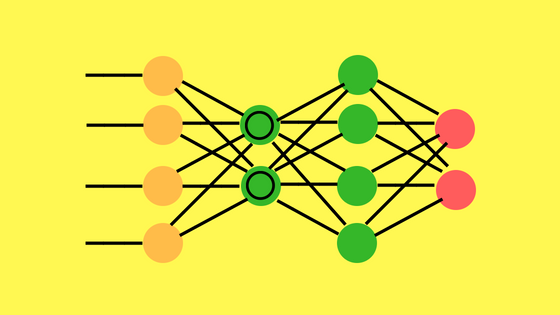
\includegraphics[width=0.25\textwidth]{./images/deep_belief.png}
    \caption{DBN}
\end{wrapfigure}

Antes de las DBN en 2006 los modelos con "profundidad" (decenas o 
cientos de capas) eran considerados demasiado difíciles de 
entrenar (incluso con backpropagation) y el uso de las redes 
neuronales artificiales quedó estancado. Con la creación de una 
DBN que logro obtener un mejor resultado en el MNIST, se devolvió 
el entusiasmo en poder lograr el aprendizaje profundo en redes 
neuronales. Hoy en día las DBN no se utilizan demasiado, pero 
fueron un gran hito en la historia en el desarrollo del deep 
learning y permitieron seguir la exploración para mejorar las 
redes existentes CNN, LSTM, etc.

La red de creencias profundas (DBN) es un tipo de red neuronal 
profunda, que se compone de capas apiladas de máquinas de 
Boltzmann restringidas (RBM). Es un modelo generativo y fue 
propuesto por Geoffrey Hinton en 2006.

\begin{wrapfigure}{r}{0.2\textwidth} %this figure will be at the right
    \centering
    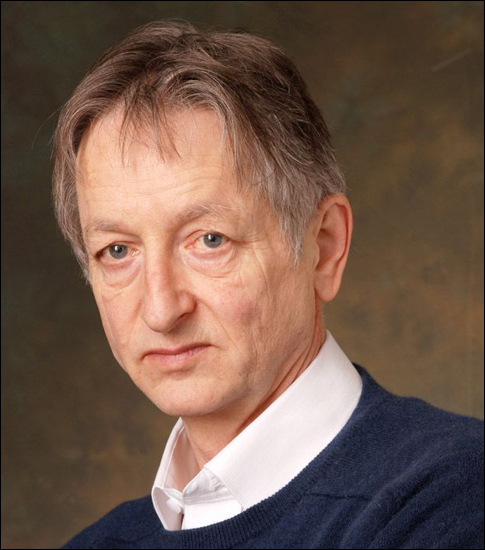
\includegraphics[width=0.2\textwidth]{./images/Geoffrey_Hinton.jpeg}
    \caption{Geoffrey Hinton}
\end{wrapfigure}

Geoffrey Everest Hinton (nacido el 6 de diciembre de 1947) es un 
psicólogo cognitivo e informático británico-canadiense, más 
conocido por su trabajo en redes neuronales artificiales. Desde 
2013, divide su tiempo trabajando para Google (Google Brain) y la 
Universidad de Toronto. En 2017, cofundó y se convirtió en el 
principal asesor científico del Vector Institute en Toronto\cite{wikigeoffrey}.

Con David Rumelhart y Ronald J. Williams, Hinton fue coautor de un 
artículo muy citado publicado en 1986 que popularizó el algoritmo 
de retropropagación para entrenar redes neuronales multicapas, 
aunque no fueron los primeros en proponer el enfoque. Hinton es 
visto como una figura destacada en la comunidad de aprendizaje 
profundo. El espectacular hito del reconocimiento de imágenes de 
AlexNet diseñado en colaboración con sus alumnos Alex Krizhevsky e 
Ilya Sutskever para el desafío ImageNet 2012 fue un gran avance en 
el campo de la visión por computadora.
Hinton recibió el Premio Turing 2018, junto con Yoshua Bengio y 
Yann LeCun, por su trabajo en aprendizaje profundo y han seguido 
dando charlas públicas juntos.

Las Deep Belief Networks, demostraron que utilizar pesos 
aleatorios al inicializar las redes son una mala idea: por ejemplo 
al utilizar Backpropagation con Descenso por gradiente muchas 
veces se caía en mínimos locales, sin lograr optimizar los pesos. 
Mejor será utilizar una asignación de pesos inteligente mediante 
un preentrenamiento de las capas de la red -en inglés “pretrain”-. 
Se basa en el uso de la utilización de Restricted Boltzmann 
Machines y Autoencoders para pre-entrenar la red de manera no 
supervisada. Ojo! luego de pre-entrenar y asignar esos pesos 
iniciales, deberemos entrenar la red por de forma habitual, 
supervisada (por ejemplo con backpropagation).

Se cree que ese preentrenamiento es una de las causas de la gran 
mejora en las redes neuronales y permitir el deep learning: pues 
para asignar los valores se evalúa capa a capa, de a una, y no 
"sufre" de cierto sesgo que causa el backpropagation, al entrenar 
a todas las capas en simultáneo.

\section{Generatives Adversarial Networks}
\begin{center}

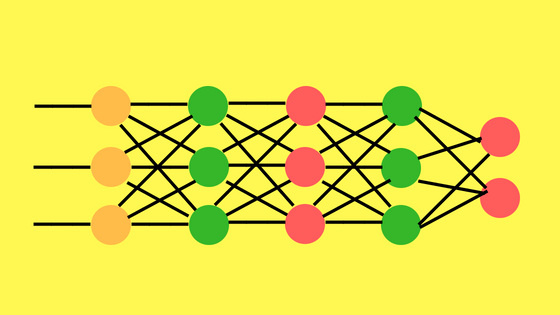
\includegraphics[scale=0.5]{./images/gan.png}

\end{center}
\subsection{Algoritmos Generativos vs. Discriminatorios}

Para entender las GAN, hay que saber cómo funcionan los algoritmos 
generativos y, para ello, es útil contrastarlos con los llamados 
algoritmos discriminatorios. Los algoritmos discriminatorios 
tratan de clasificar los datos de entrada. Es decir, dadas unas 
características de unos datos, predicen una etiqueta o categoría a 
la que pertenecen esos datos. Por ejemplo, dadas todas las palabras 
de un correo electrónico un 
algoritmo discriminatorio podría predecir si el mensaje es `spam' 
o `no spam'. Spam es una de las etiquetas, y la `bolsa de 
palabras' recopiladas del correo electrónico son las 
características que constituyen los datos de entrada.

Así que los algoritmos discriminatorios asignan características a 
las etiquetas. Se refieren únicamente a esa correlación. Una forma 
de pensar en los algoritmos generativos es que hacen precisamente 
lo contrario; en lugar de predecir una etiqueta con ciertas 
características, intentan predecir características con una 
etiqueta determinada.

Por eso la pregunta que un algoritmo generativo intenta responder 
es:

``¿Asumiendo que este correo electrónico es spam, ¿Cómo de 
probable es que sean estas características?''

\subsection{Nacimiento de las GAN}

Una noche de 2014, Ian Goodfellow fue a beber para celebrar con un 
estudiante de doctorado que acababa de graduarse. A
Les 3 Brasseurs (Los tres cerveceros), un abrevadero favorito de 
Montreal, algunos amigos le pidieron ayuda con un proyecto 
bastante desafiante en el que estaban trabajando: un programa que 
podía crear fotos por sí mismo\cite{techreview}.

Los investigadores ya estaban usando redes neuronales como
modelos "generativos" para crear nuevos datos plausibles propios. 
Pero los resultados a menudo no eran muy buenos: las imágenes de 
un rostro generado por computadora tendía a ser borroso o a tener 
errores como orejas faltantes. El plan que tenían los amigos de 
Goodfellow era utilizar un análisis estadístico complejo de los 
elementos que componen una fotografía para ayudar a las máquinas a 
crear
con imágenes por sí mismos. Esto habría requerido una gran 
cantidad de cálculos numéricos, y Goodfellow les dijo que
simplemente no iba a funcionar.

Pero mientras reflexionaba sobre el problema con su cerveza, se le 
ocurrió una idea. ¿Qué pasa si enfrentas dos redes neuronales una 
contra la otra? Sus amigos estaban escépticos, así que una vez que 
llegó a casa, donde su novia ya estaba profundamente dormida, 
decidió
darle una oportunidad. Goodfellow codificó en las primeras horas y 
luego probó su software y este funcionó a la primera.

Lo que inventó esa noche ahora se llama GAN, o ``red antagónica 
generativa''. La técnica ha despertado gran
entusiasmo en el campo del aprendizaje automático y convirtió a su 
creador en una celebridad de la IA.

En los últimos años, los investigadores de IA han logrado un 
progreso impresionante utilizando una técnica llamada aprendizaje 
profundo. Suministre a un
sistema de aprendizaje profundo con suficientes imágenes y aprende 
a, por ejemplo, reconocer a un peatón que está a punto de cruzar 
una calle. Este enfoque ha hecho posibles cosas como los autos sin 
conductor y la tecnología conversacional que impulsa a Alexa, Siri 
y otros asistentes virtuales.

Pero si bien las IA de aprendizaje profundo pueden aprender a 
reconocer cosas, no han sido buenas para crearlas. El objetivo de 
las GAN es dar a las máquinas algo parecido a la imaginación.

En el futuro, las computadoras serán mucho mejores para darse un 
festín con los datos sin procesar que hay por todo el mundo, la ya 
famosa Big Data, y descubrir lo que necesitan aprender de ellos.

Hacerlo no solo les permitiría hacer dibujos bonitos o componer 
música; los haría menos dependientes de los humanos
para instruirlos sobre el mundo y la forma en que funciona. Hoy en 
día, los programadores de IA a menudo necesitan decirle a una 
máquina exactamente qué hay en los datos de entrenamiento de los 
cuales se están alimentando: cuáles de ese millón de imágenes 
contienen un peatón cruzando una calle y cuáles
no. Esto no solo es costoso y requiere mucha mano de obra sino que 
también limita qué tan bien el sistema maneja incluso las 
desviaciones leves de lo que ya fue entrenado. En el futuro, las 
computadoras serán mucho mejores para deleitarse con datos sin 
procesar y resolver qué necesitan aprender de ellos sin que se les 
diga.

 Un coche autónomo podría enseñarse a si mismo sobre muchas 
 condiciones diferentes de la carretera sin salir del garaje. Un 
 robot podría anticipar los obstáculos que podría encuentrar en un 
 almacén concurrido sin necesidad de que lo lleven.

Eso marcará un gran salto adelante en lo que se conoce en IA como 
``aprendizaje no supervisado''.

Nuestra capacidad de imaginar y reflexionar sobre muchos 
escenarios diferentes es parte de lo que nos hace humanos. Y 
cuando los futuros historiadores de la tecnología miren hacia 
atrás, es probable que vean las GAN como un gran paso hacia la 
creación de máquinas con una conciencia similar a la humana. Yann 
LeCun, científico jefe de IA de Facebook, ha llamado a las GAN “la 
mejor idea en aprendizaje profundo en los últimos 20 años.” 

Otro grande de la IA, Andrew Ng, ex científico jefe de Baidu de 
China, dice que los GAN representan ``un
avance significativo y fundamental'' que inspiró a una creciente 
comunidad global de investigadores.

\subsection{Ian Goodfellow, el padre de las GAN}

\begin{wrapfigure}{r}{0.25\textwidth} %this figure will be at the right
    \centering
    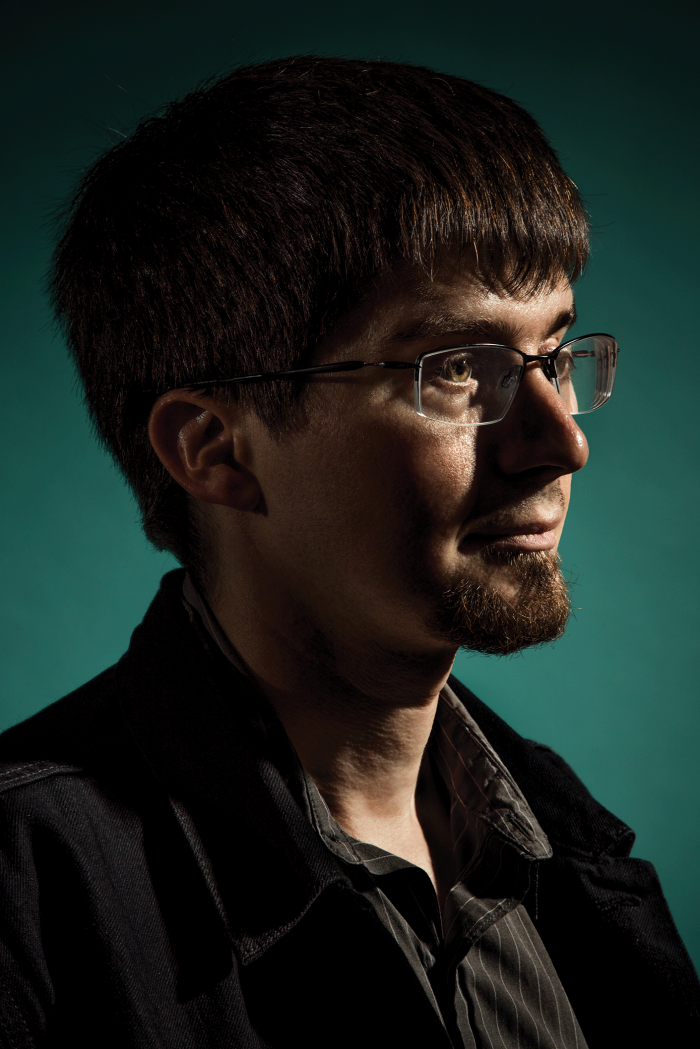
\includegraphics[width=0.25\textwidth]{./images/ma18-iangoodfellow2a.png}
    \caption{``Ian Goodfellow''}
\end{wrapfigure}


Goodfellow ahora es científico investigador en el equipo de Google 
Brain, en la sede de la compañía en Mountain View,
California. Todavía está sorprendido por su estatus de 
superestrella, calificándolo de ``un poco surrealista''. Quizás lo 
menos sorprendente es que, después de haber hecho su 
descubrimiento, ahora pasa gran parte de su tiempo tra5bajando 
contra aquellos que desean usarlo para fines malvados.

La magia de las GAN radica en la rivalidad entre las dos redes 
neuronales. Imita el tira y afloja entre un falsificador de 
imágenes y un detective de arte que repetidamente intentan 
burlarse entre ellos. Ambas redes están entrenadas en el mismo 
conjunto de datos. El primero, conocido como generador, se encarga 
de producir resultados artificiales, como fotos o escritura a 
mano, que sean lo más realistas posible. El segundo, conocido como 
el discriminador, los compara con imágenes genuinas del conjunto 
de datos original e intenta determinar cuáles son reales y cuáles 
son falsos. Sobre la base de esos resultados, el generador ajusta 
sus parámetros para crear nuevas imágenes. Y así sigue, hasta que 
el discriminador ya no puede decir lo que es genuino y lo que es 
falso.
En un ejemplo ampliamente publicitado el año pasado, los 
investigadores de Nvidia, una empresa de chips que invirtió mucho 
en IA, entrenaron una GAN para generar imágenes de celebridades 
imaginarias mediante el estudio de las reales. No todas las 
estrellas falsas que produjo fueron perfectas, pero algunas fueron 
impresionantemente realistas. A diferencia de otros enfoques de 
aprendizaje automático que requieren decenas de miles de imágenes 
de entrenamiento, las GAN pueden volverse competentes con unos 
pocos cientos.

Este poder de la imaginación es todavía limitado. Una vez que ha 
sido entrenado en muchas fotos de perros, un GAN puede generar un
imagen falsa convincente de un perro que tiene, digamos, un patrón 
diferente de manchas; pero no puede concebir un completamente 
nuevo animal. La calidad de los datos de entrenamiento originales 
también tiene una gran influencia en los resultados. En un ejemplo 
revelador, un GAN comenzó a producir imágenes de gatos con letras 
aleatorias integradas en las imágenes. Porque los datos de 
entrenamiento contenía memes de gatos de Internet, la máquina se 
había enseñado a sí misma que las palabras eran parte de lo que 
significaba ser un gato.

Las GAN también son temperamentales, dice Pedro Domingos, 
investigador de aprendizaje automático de la Universidad de 
Washington. Si el
discriminador es demasiado fácil de engañar, la salida del 
generador no se verá realista. Y calibrar los dos modelos 
neurales puede llegar a ser difícil, lo que explica por qué las 
GAN a veces escupen cosas extrañas, como animales con dos cabezas.

Aún así, los desafíos no han disuadido a los investigadores. Desde 
que Goodfellow y algunos otros publicaron el primer estudio sobre 
su descubrimiento, en 2014, se han escrito cientos de artículos 
relacionados con GAN. Un fanático de la tecnología incluso ha 
creado una web página llamada ``Zoológico GAN'', dedicada a 
realizar un seguimiento de las diversas versiones de la técnica 
que se han desarrollado.

Las aplicaciones inmediatas más obvias se encuentran en áreas que 
involucran muchas imágenes, como los videojuegos y la moda:
¿Cómo, por ejemplo, se vería un personaje de un juego corriendo 
bajo la lluvia? Pero de cara al futuro, Goodfellow cree que las 
GAN impulsarán avances más significativos. “Hay muchas áreas de la 
ciencia y la ingeniería en las que debemos
optimizar algo”, dice, citando ejemplos como medicamentos que 
necesitan ser más efectivos o baterías que deben
ser más eficiente. “Esa va a ser la próxima gran ola”.

En la física de alta energía, los científicos usan poderosas 
computadoras para simular las probables interacciones de cientos 
de partículas subatómicas en máquinas como el Gran Colisionador de 
Hadrones en el CERN en Suiza. Estas simulaciones son lentas y 
requieren poder de cómputo masivo. Investigadores de la 
Universidad de Yale y el Laboratorio Nacional Lawrence Berkeley 
han desarrollado una GAN que, después de entrenarse con los datos 
de simulación existentes, aprende a generar predicciones bastante 
precisas de cómo se comportará una partícula en particular, y lo 
hace mucho más rápido.

\begin{wrapfigure}{l}{0.5\textwidth} %this figure will be at the right
    \centering
     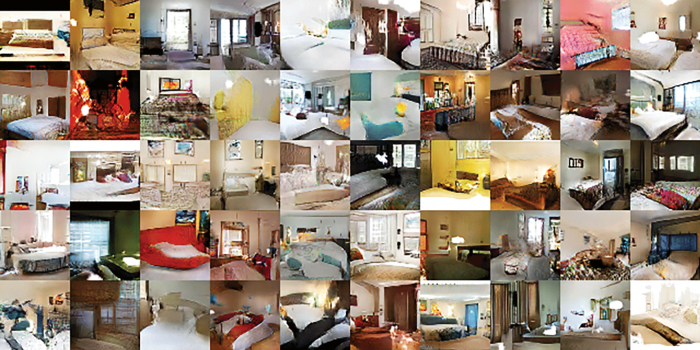
\includegraphics[width=0.5\textwidth]{./images/interiores.png}
	  \caption{``La creación de Goodfellow se puede utilizar para imaginar todo tipo de cosas, incluidos nuevos diseños de interiores.''}
\end{wrapfigure}




La investigación médica es otro campo prometedor. Las 
preocupaciones de privacidad significan que los investigadores a 
veces no pueden obtener suficientes datos reales de pacientes 
para, por ejemplo, analizar por qué un medicamento no funcionó. 
Las GAN pueden ayudar a resolver este problema al generar 
registros falsos que son casi tan buenos como los reales, dice 
Casey Greene de la Universidad de Pensilvania. Estos datos podrían 
compartirse más ampliamente, ayudando a avanzar en la 
investigación, mientras que los registros reales están 
estrictamente protegidos.
\begin{wrapfigure}{r}{0.3\textwidth} %this figure will be at the right
    \centering
     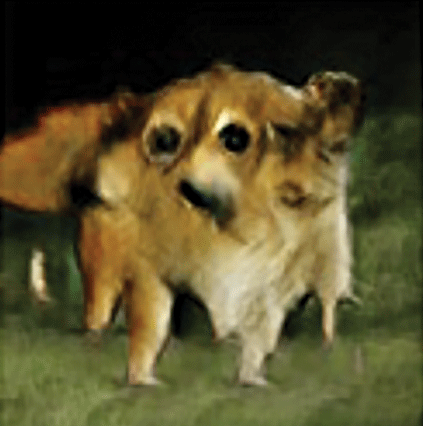
\includegraphics[width=0.3\textwidth]{./images/rares_images.png}
	  \caption{``Hacer que las GANs funcionen bien puede ser complicado. Si hay fallas, los resultados pueden ser extraños.''(Alec Radford)}
\end{wrapfigure}
Sin embargo, hay un lado más oscuro. Una máquina diseñada para 
crear falsificaciones realistas es un arma perfecta para los 
proveedores de noticias falsas que quieren influir en todo, desde 
los precios de las acciones hasta las elecciones. Las herramientas 
de IA ya se están utilizando para poner imágenes de rostros de 
otras personas en los cuerpos de estrellas del cine adulto y poner 
palabras en la boca de los políticos. Las GAN no crearon este 
problema, pero lo empeorarán.
 
 Hany Farid, que estudia ciencia forense digital en Dartmouth 
 College, está trabajando en mejores formas de detectar videos  
 falsos, como detectar cambios leves en el color de los rostros  
 causados por la inhalación y la exhalación que las GAN encuentran 
 difíciles de imitar con precisión. Pero advierte que las GAN se  
 adaptarán a su vez. ``Estamos fundamentalmente en una posición  
 débil'', dice Farid.



Este juego del gato y el ratón también se desarrollará en la 
ciberseguridad. Los investigadores ya están destacando el riesgo 
de los ataques de ``caja negra``, en los que las GAN se utilizan 
para descubrir los modelos de aprendizaje automático con los que 
muchos programas de seguridad detectan el malware. Habiendo 
adivinado cómo funciona el algoritmo de un defensor, un atacante 
puede evadirlo e insertar código malicioso. El mismo enfoque 
también podría usarse para esquivar los filtros de spam y otras 
defensas.

``Hay muchas áreas de la ciencia y la ingeniería en las que 
necesitamos optimizar algo. Esa va a ser la próxima gran ola''.

Goodfellow es muy consciente de los peligros. Ahora, al frente de 
un equipo en Google que se enfoca en hacer que el aprendizaje 
automático sea más seguro, advierte que la comunidad de IA debe 
aprender la lección de las oleadas de innovación anteriores, en 
las que los tecnólogos trataron la seguridad y la privacidad como 
una idea de último momento. Cuando se dieron cuenta de los 
riesgos, los malos tenían una ventaja significativa. ``Claramente, 
ya estamos más allá del comienzo'', dice, ``pero con suerte 
podemos lograr avances significativos en seguridad antes de que 
nos adentremos demasiado''.

Sin embargo, no cree que haya una solución puramente tecnológica 
para la falsificación. En su lugar, cree, tendremos que depender 
de las sociales, como enseñar a los niños el pensamiento crítico 
al hacer que tomen cosas como clases de oratoria y debate. ``En 
oratoria y debate, estás compitiendo contra otro estudiante'', 
dice, ``y estás pensando en cómo elaborar afirmaciones engañosas o 
cómo elaborar afirmaciones correctas que sean muy persuasivas''. 
Puede que tenga razón, pero su conclusión de que la tecnología no 
puede curar el problema de las noticias falsas no es algo que 
muchos quieran escuchar.

\begin{thebibliography}{9}


\bibitem[WIKI GAN]{wikigan}
es.wikipedia.org. 2022. Red generativa antagónica - Wikipedia, la enciclopedia libre. Disponible en: \url{https://es.wikipedia.org/wiki/Red_generativa_antagónica} Accedido 15 junio 2022.

\bibitem[RAPIDMINER]{rapidminer}
RapidMiner. 2022. Generative Adversarial Network (GANs) | RapidMiner. Disponible en: \url{https://rapidminer.com/glossary/generative-adversarial-networks} Accedido 15 junio 2022.

\bibitem[TECHREVIEW]{techreview}
MIT Technology Review. 2018. The GANfather: The man who’s given machines the gift of imagination. Disponible en: \url{https://www.technologyreview.com/2018/02/21/145289/the-ganfather-the-man-whos-given-machines-the-gift-of-imagination} Accedido 15 junio 2022].

\bibitem[PUENTESDIGIT]{puentesdigit}
Puentesdigitales.com. 2019. Todo lo que necesitas saber sobre las GAN: Redes Generativas Antagónicas – Puentes Digitales. Disponible en: \url{https://puentesdigitales.com/2019/04/05/todo-lo-que-necesitas-saber-sobre-las-gan-redes-generativas-antagonicas} Accedido 15 junio 2022.

\bibitem[WIKI LOGIT]{wikilogit}
En.wikipedia.org. 2022. Logistic regression - Wikipedia. Disponible en: \url{https://en.wikipedia.org/wiki/Logistic_regression} Accedido 15 junio 2022.

\bibitem[WIKI PERCEPT]{wikipercept}
Es.wikipedia.org. 2022. Perceptrón - Wikipedia, la enciclopedia libre. Disponible en: \url{https://es.wikipedia.org/wiki/Perceptrón} Accedido 15 junio 2022.

\bibitem[WIKI MULTILAYER]{wikimultilayer}
Es.wikipedia.org. 2022. Perceptrón multicapa - Wikipedia, la enciclopedia libre. Disponible en: \url{https://es.wikipedia.org/wiki/Perceptrón_multicapa} Accedido 15 junio 2022.

\bibitem[WIKI FRANK]{wikifrank}
Es.wikipedia.org. 2022. Frank Rosenblatt - Wikipedia, la enciclopedia libre. Disponible en: \url{https://es.wikipedia.org/wiki/Frank_Rosenblatt} Accedido 15 junio 2022.

\bibitem[WIKI YANN]{wikiyann}
Es.wikipedia.org. 2022. Yann LeCun - Wikipedia, la enciclopedia libre. Disponible en: \url{https://es.wikipedia.org/wiki/Yann_LeCun} Accedido 15 junio 2022.

\bibitem[WIKI GEOFFREY]{wikigeoffrey}
En.wikipedia.org. 2022. Geoffrey Hinton - Wikipedia. Disponible en: \url{https://en.wikipedia.org/wiki/Geoffrey_Hinton} Accedido 15 junio 2022.

\bibitem[WIKI PIERRE]{wikipierre}
En.wikipedia.org. 2022. Pierre François Verhulst - Wikipedia. Disponible en: \url{https://en.wikipedia.org/wiki/Pierre_François_Verhulst} Accedido 15 junio 2022.

\bibitem[A BRIEF HISTORY]{history}
Skynet Today. 2022. A Brief History of Neural Nets and Deep Learning. Disponible en: \url{https://www.skynettoday.com/overviews/neural-net-history} Accedido 15 junio 2022.

\end{thebibliography}
\newpage
\tableofcontents
\end{document}
